\section {Architecture Overview}

\begin{figure}[!t]
  \centering
  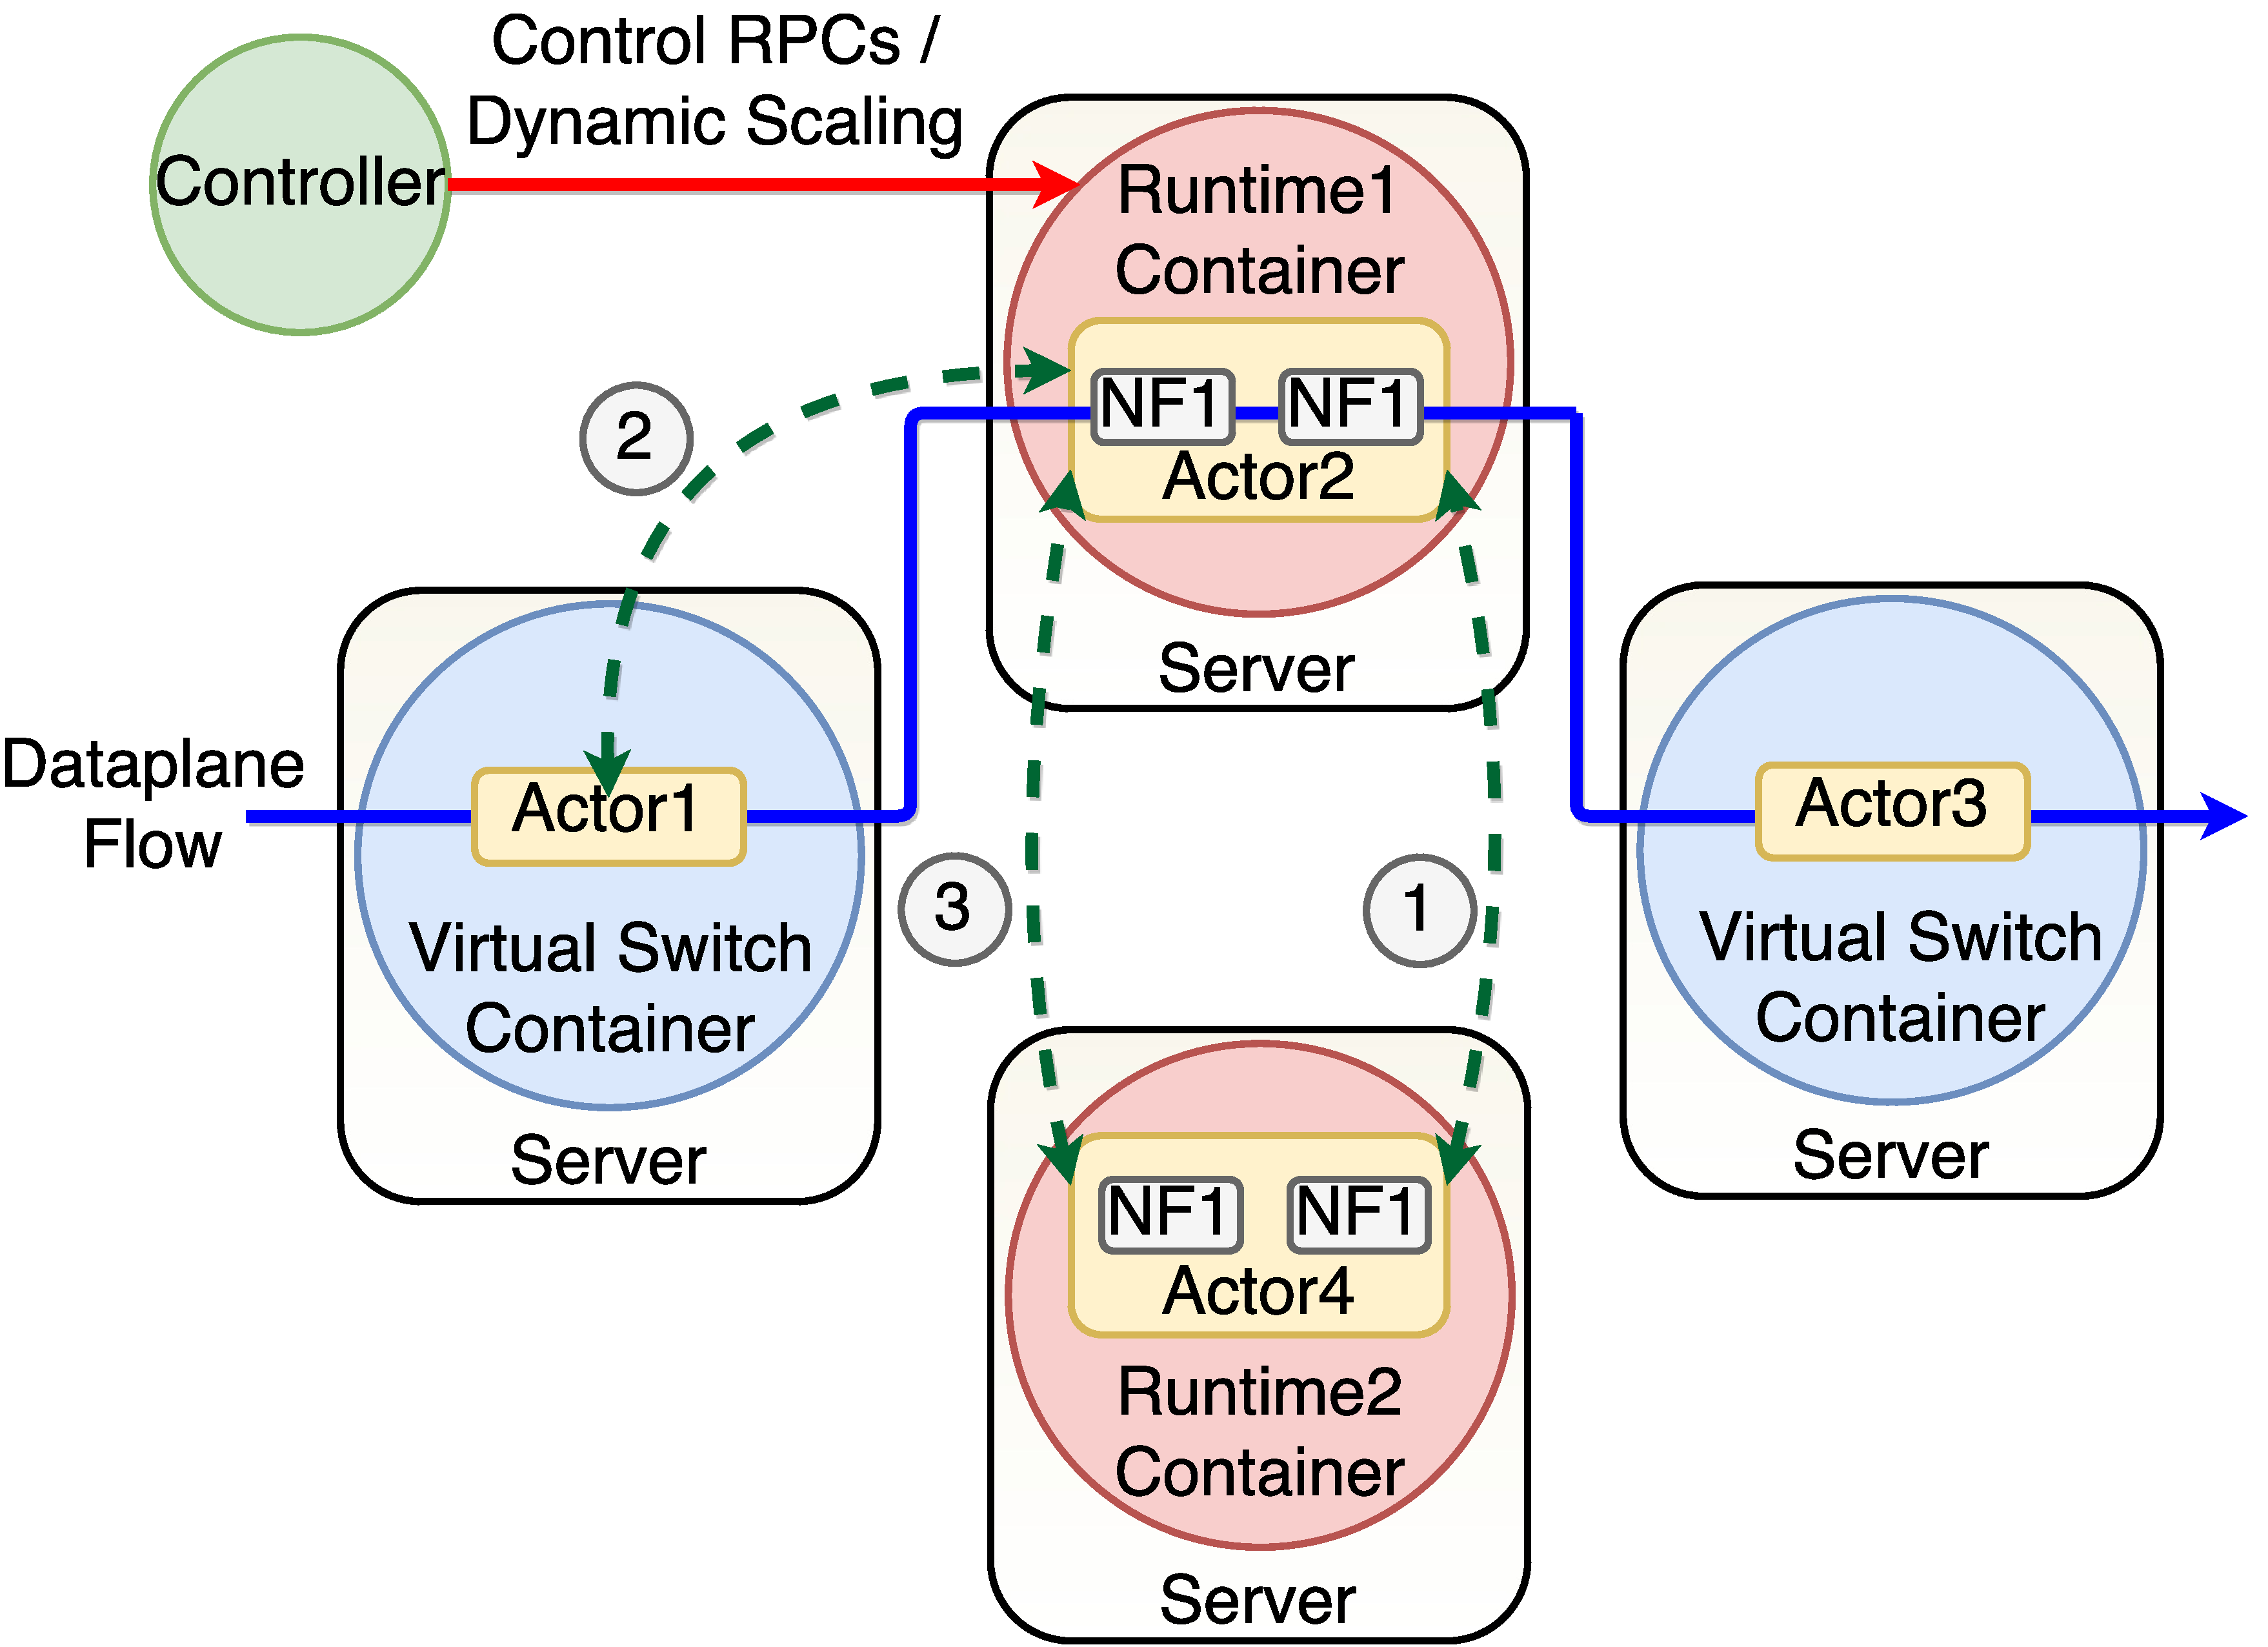
\includegraphics[width=\columnwidth]{figure/final-final-nfactor-cluster.pdf}
  \caption{An overview of NFActor framework.}
  \label{fig:runtime}
\end{figure}

Figure \ref{fig:runtime} demonstrates the basic architecture of NFActor framework, consisting of a light-weight controller, input and output virtual switches and several runtime systems (referred to as \textit{runtime} in short). NFActor framework runs virtual switches and runtimes inside containers, so that they can be quickly rebooted in case of failure and elastically scaled in case of overload.

The incoming dataplane flows are first sent to the input virtual switch, which dispatches them to runtimes. Each runtime hosts a NF service chain that is determined during runtime initialization phase and conducts the actual serivce chain processing. When a runtime receives a new flow, it creates a new actor and delegates the packet processing of the flow to that actor. The actor loads all the required NF modules of the service chain when it is created and passes the received flow packet to these NF modules in sequence. Once the service chain processing is finished, the actor sends the packet to an output virtual switch, where the packet is sent to its final destination.

The key feature that differentiates NFActor framework with existing works like \cite{gember2015opennf} and \cite{rajagopalan2013split} is that flow mif
One of most significant features that differentiate NFActor framework with existing works \cite{gember2015opennf} is that flow management tasks is fully automated without the need of a centralized controller. In figure \ref{fig:runtime}, actor 2 in runtime 1 could migrate itself to actor 4 on runtime 2, by exchanging 3 messages with actor 1 and actor 4. The decentralized nature of NFActor framework originates the micro execution context built for each flow.

A controller does exists in NFActor framework, which is a relatively light-weighted one. It's tasks are to monitor the workload of each runtime and control dynamic scaling. It's only appearance when executing flow management tasks is during the initiation phase, where it uses control RPCs to tell the flows which runtime they should migrate to.
